%%%%%%%%%%%%%%%%%%%%%%%%%%%%%% -*- Mode: Latex -*- %%%%%%%%%%%%%%%%%%%%%%%%%%%%
%% project.tex -- 
%% Author          : Philip Johnson
%% Created On      : Tue Mar 31 11:44:58 2009
%% Last Modified By: Philip Johnson
%% Last Modified On: Wed Jan 18 11:09:27 2012
%%%%%%%%%%%%%%%%%%%%%%%%%%%%%%%%%%%%%%%%%%%%%%%%%%%%%%%%%%%%%%%%%%%%%%%%%%%%%%%

\documentclass{proposalnsf}
\usepackage[final]{graphicx}
\usepackage{url}

% NSF proposal generation template style file.
% based on latex stylefiles  written by Stefan Llewellyn Smith and
% Sarah Gille, with contributions from other collaborators.

\renewcommand{\refname}{\centerline{References cited}}

% Fix things so that figures tend to stay away from the last page. 
\renewcommand{\topfraction}{0.85}
\renewcommand{\textfraction}{0.1}
\renewcommand{\floatpagefraction}{0.75}

% this handles hanging indents for publications
\def\rrr#1\\{\par
\medskip\hbox{\vbox{\parindent=2em\hsize=6.12in
\hangindent=4em\hangafter=1#1}}}

\def\baselinestretch{1}

\renewcommand{\thefootnote}{}

\begin{document}



% \pagenumbering{arabic}
% \renewcommand{\thepage} {C--\arabic{page}}
% \renewcommand{\thesection} {C.\arabic{section}}
% \setcounter{section}{0}

\section{Project Description}

\tableofcontents

\input{01.project.intro}

\subsection{Pathway to Smart, Sustainable Microgrids} 

Our pathway to smart, sustainable microgrids involves the development of a testbed consisting
of the UH Manoa campus.  This section goes into detail on the five research
components introduced above. 

\input{02.project.sensing}

%%%%%%%%%%%%%%%%%%%%%%%%%%%%%% -*- Mode: Latex -*- %%%%%%%%%%%%%%%%%%%%%%%%%%%%
%% project.modeling.tex --
%% Author          : Philip Johnson
%% Created On      : Fri Jan 13 07:58:21 2012
%% Last Modified By: Philip Johnson
%% Last Modified On: Thu Jan 26 13:11:43 2012
%%%%%%%%%%%%%%%%%%%%%%%%%%%%%%%%%%%%%%%%%%%%%%%%%%%%%%%%%%%%%%%%%%%%%%%%%%%%%%%

\subsubsection{Research component: Modeling and analysis}
\label{sec:modeling}

Given appropriate data, the next step is to apply analytic techniques to
create real-time and historical information useful for control and
optimization of the microgrid.

Two important contributions of this part of the research will be: (1) analytic techniques that enable us to adequately characterize the current state of the microgrid while minimizing cost-prohibitive deployment of sensing equipment, and (2) analytic techniques that enable short-term prediction of various useful attributes of the micro-grid (such as future potentially peak load and ramp) and the surrounding environment (insolation, wind speed and direction, etc.)  

It should be noted that there is an interdependence between the ``sensing
and monitoring'' subproject and the ``modeling and analysis'' subproject:
we will ``tune'' the installation of sensing equipment in order to obtain
acceptable quality of analytic outcomes for the next step, control and
optimization. Furthermore, the chosen models and analytical tools cannot
only be good descriptors of the underlying physical processes, but also
need to be matched to the signal processing (detection and estimation)
methods, or else the signal processing methods will not be of much use.


\begin{figure}[th!]
  \begin{center}
   \includegraphics[width=0.6\textwidth]{fig/Bipartite.eps}
   \caption{\label{B} Factor graph - an abstraction of the microgrid.
       The factor graph consists
       of the behavior layer and the observation layer. The
       communication layer provides additional global
       communication features. In this figure, the state
       variables are denoted by $x_i$ and available observations
       (sparse measurements) are denoted by $y_i$.
       The belief-propagation algorithm is
       a monitoring algorithm that works by passing only {\em local}
       messages along the solid edges of the graph, yet achieves {\em global}
       monitoring.}
  \end{center}
\end{figure}

\paragraph{Belief Propagation.} Through or previously funded NSF project
(ECCS-1029081), we have already established that the factor-graph approach
is well-suited to modeling the electrical connections of a microgrid.
Figure~\ref{B} shows a schematic view of a factor-graph associated with a
fictitious microgrid. The nodes in the mocrogrid are divided into three
layers: 1) the observation layer (sensors, measurement equipment), 2) the
behavior layer (collection of network nodes, loads and microgenerators) and
3) the communication layer. We demonstrated that, with only a few well
placed sensors in the grid, we are able to track slowly evolving behaviors
of the grid as well as with more elaborate exact maximum-likelihood
estimators~\cite{Hu10,Hu11,Hu11a}. This is mainly because the electrical
grid is typically a {\em tree} graph, where correlations among renewable
sources create rare loops with large diameters.

In this research, we plan to use belief propagation as a tool that would
also enable 1) tracking the grid in transitional modes (e.g., if a large
number of users and/or renewable microgenerators enter and/or drop from the
microgrid abruptly) and 2) short-term future prediction of the grid
behavior at node-levels.  To this end, we will develop the necessary
modeling and prediction tools.

\paragraph{Modeling demand.} Often, the demand in grid networks is
described using historical {\em histograms}. However, historical histogram
patterns do not reveal the true spatiotemporal character of the demand. It
is obvious that spatial and temporal correlations will need to be exploited
in order to arrive at a model that would be useful for spatiotemporal
demand prediction, i.e., prediction that can predict the demand, say, five
minutes in advance at any given set of spatial location locations in the
microgrid.  Furthermore, in order to utilize the belief-propagation tool,
we will seek to model the demand among various nodes in the microgrid as a
spatiotemporal Markov process with as few loops as possible (because it is
the loops that adversely affect belief
propagation~\cite{Wiberg95,Kschischang01,Loeliger07}). We note that simple
Gauss-Markov process modeling will likely not suffice because Gaussian
processes are well-suited only for tracking slow changes.  Yet, demand in
campus environment can be spatially and temporally bursty (because of
correlation to class-time starts, lab-clusters, weather/heat conditions and
distributed renewable microgenerators).  For this reason, we plan to leverage
our experience in modeling Gauss-Markov processes~\cite{Kavcic00a} and
finite-state machines~\cite{Yang05,Vontobel08} to develop a comprehensive
double-layer Gauss-Markov/finite-state spatiotemporal demand model.  We
will extrapolate, calibrate and test the model using measurement data from
sensors distributed around the campus.

\paragraph{Modeling renewable sources.} Much like the loads (demand) are spatially and temporally distributed, so are the renewable micro-generators. The UH campus already has several photovoltaic (PV) systems and two small wind turbines (used for experimental purposes) dispersed around campus.  Therefore, we will need to begin by modeling their energy outputs using spatiotemporal Markov processes (with as few loops as possible) that are capable of modeling both slowly varying effects as well as (spatially and temporally) localized bursts. Again, we will utilize a layered Gauss-Markov/finite-state modeling approach to capture both effects. However, unlike modeling demand, here we will need to heavily correlate the model to weather conditions (night/day, cloud-cover, wind speed and direction). We will extrapolate, calibrate and test the model using weather measurement data from irradiance sensors, wind velocity sensors and cloud cameras distributed around the campus.

\paragraph{Prediction.} It is a well-known fact that the Kalman predictor
is the optimal predictor of spatial and temporal Gaussian
processes~\cite{Kalman60,Kalman_Bucy61,Kailath68}. When the Gaussian
process further possesses a Markov structure (i.e., a Gauss-Markov
process), the Kalman predictor is computationally less
intensive~\cite{Kschischang01,Loeliger07}. In our case, we will
likely have a two-layer spatial and temporal
Gauss-Markov/finite-state process to track. The optimal tracker of
this process would be a spatiotemporal combination of a Kalman
predictor~\cite{Kalman60,Kalman_Bucy61} and a forward recursion of
the Baum-Welch algorithm~\cite{Baum66,Bahl74}. However, this
approach will likely be too computationally intensive to be
practical. Therefore, we will ignore the loops in the model, and
implement the predictor using belief propagation derived for a
tree-like double-layer (Gauss-Markov/finite-state) graph, but
applied to the exact loopy microgrid graph.

We envision that the developed prediction tool will be used to
indicate where and how the control mechanisms (e.g., peak-shaving,
gray-outs, etc.) should be applied. However, we must consider the
sensitivity of certain locations when applying control.  For
example, it would be detrimental to shut off the air conditioner in
a sensitive climate controlled laboratory, or in computer server
clusters that must remain cool. For this reason, it is desirable to
have a prediction method that will account for these sensitivities.
It is well-known that any prediction method suffers form
uncertainly, misdetection and false alarms. Grossly false estimation
or prediction of the state of certain sensitive nodes may adversely
affect the stability of the network or sensitive campus locations.
This can be minimized in two possible ways. Firstly, we may choose
to place sensors in the vicinities of highly sensitive nodes, and
thus minimize the risk of misprediction. Secondly, we may choose to
dampen the belief-propagation algorithm to prevent wild belief
swings in the vicinities of highly sensitive nodes. This amounts to
placing weights (or other types of constraints) on beliefs
corresponding to highly sensitive nodes. We shall term this approach
{\em sensitivity weighted} belief-propagation. To our knowledge, no
such approach has been attempted in smart-grid networks, although
similar strategies are available in the communications and
error-control coding literature~\cite{Wang99,Jiang06a,Varnica07}.

\paragraph{Analysis.} The final piece of the modeling and analysis effort is the actual analysis of the proposed models and tracking methods. In tracking mode, we will utilize statistical signal processing techniques to analyze the performance of the trackers. For example, under stationarity conditions, we can easily bound the performance of maximum-likelihood estimators of Gaussian processes. We will extend these
techniques, and combine them with bounding techniques typical for
finite-state processes~\cite{Huang09}, to develop bounds for tracking the
layered Gauss-Markov/finite-state process  under certain stationarity assumptions.

Under extremely non-stationary, non-Gaussian conditions, however, it will be extremely difficult to come up with analytical tools that will be able to bound the performance of the estimator/tracker. Indeed, in the signal processing literature, response to extreme non-stationarities are typically demonstrated by simulations ~\cite{Yang95,Tanaka05}. For this reason, it is actually
very important to design a robust model that will not only be useful
for designing the detector, but also for designing the simulator.
The usefulness of this approach will be extremely important when
determining the response to {\em rare or contingency events}. Rare events are
events that are rarely (or never observed) in practice until they
happen in reality (e.g., black-outs, shut-downs, catastrophic
failures, storms). The only way to understand how such events would affect
the system is through simulations. We will conduct analysis studies
of these rare, extremely non-stationary events through the means of
simulations using the developed process models.


\input{04.project.control}

\input{05.project.social}

%%%%%%%%%%%%%%%%%%%%%%%%%%%%%% -*- Mode: Latex -*- %%%%%%%%%%%%%%%%%%%%%%%%%%%%
%% project.workforce.tex -- 
%% Author          : Philip Johnson
%% Created On      : Fri Jan 13 07:58:21 2012
%% Last Modified By: Philip Johnson
%% Last Modified On: Thu Jan 26 15:31:53 2012
%%%%%%%%%%%%%%%%%%%%%%%%%%%%%%%%%%%%%%%%%%%%%%%%%%%%%%%%%%%%%%%%%%%%%%%%%%%%%%%

\subsubsection{Research component: Education and workforce development}
\label{sec:education}
  
The Hawaii Clean Energy Initiative (HECI) is a Memorandum of 
Understanding (MOU) between the state of  Hawaii and
the Department of Energy signed in 2008 that set goals for Hawaii so that by 2030
70\% of our energy will come from clean energy sources
(30\% from energy efficiency and 40\% from renewable energy sources).   
Through  the Renewable Energy and Island Sustainability (REIS) goup  we have developed 
curriculum and courses in energy and sustainability to help train this workforce that will be
needed to achieve these goals.  Much as HCEI will rely more on local energy sources the
REIS group is working to have Hawaii more reliant on locally trained experts in energy and
sustainability.

At  the UHM we are developing multidisciplinary education and research programs that span the range of jobs that will be needed to supply new educated workforce in the energy and sustainability areas.  We have funded workforce training programs at the University of Hawai�i community college level (NSF Tribal Communities University Program (TCUP) Pre-Engineering Education Collaborative (PEEC)) and at the graduate and undergraduate level at the UHM through REIS (Department of Energy (DOE) workforce training grant).   The DOE workforce training grant is
developing curriculum over a broad range of energy topics considering engineering, natural
and social science, and policy.  Student in the graduate REIS program supported by the DOE
workforce training grant take two core graduate courses in energy (one class in engineering and
the other class in social science).  The students then take other courses so that they can 
concentrate on their research which varies from studying 
nanocomposites  for fuel cells to biofuels to wave  energy to smart grid security.
  
This proposal goes one step further by focusing on an in depth understanding of microgrids,
distributed renewable energy sources, demand response, and energy efficient management.
We  will work on further development of courses in the smart grid and renewable energy
areas with a focus on systems, software, and policy issues.   We will create a variety of graduate level courses including classes on the Smart Grid and Future Electrical Energy Systems, Advanced
Software Energy Systems, and Energy Resource Assessment.  These courses will all have
engineering, economic, social,and policy aspects and provide background knowledge along
with the two core REIS graduate courses and fundamental courses in Probability, Signal Processing, Communications and Networking, Software Engineering, and Economics.  
The courses are well integrated to the four research projects and will give students a good
foundation to conduct their research.  

In addition we
are working through local funding agencies to develop a short twenty hour course on smart grids
and integration of renewable sources that will be available to UHM students and faculty and also
the external community.  This course will be broken up into five four hour segments: grid
overview,  policies and standards, tools and capabilities, communications and networking and
security, and integration of sources.

A major component of education and training is conducting research while using the Smart
Campus Energy Lab (SCEL) and working on the UHM microgrid.  Both graduate and
undergraduate students will be working on research projects in conjunction with HECO engineers
and UHM facility people.  There will be a close integration between the different research
areas and also between education in the classroom where concepts are learned, analysis where
models, algorithms, optimization, and control methods are formulated,  software and hardware
simulation studies, and the UHM campus environment 
and microgrid where analysis and simulations are confirmed.  The research projects will also educate students in team work, project management, and improve their oral and written
communication skills.

\paragraph{Integration of members of under-represented minorities}

This project will collaborate with the Native Hawaiian Science and
Engineering Mentorship Program (NHSEMP) to broaden the participation of
under-represented groups. NHSEMP is a successful program housed at the
University of Hawaii funded (in part) by the National Science Foundation
Louis Stokes Alliance for Minority Participation Program and the
U.S.~Department of Education Native Hawaiian Education Program. The program
is already very successful in attracting members of the Pacific Islander
minority into the undergraduate engineering program. Our next goal is to
achieve a smooth transition of the most talented minority students into the
best graduate programs nationwide. For example, we are already implementing
an REU exchange program with our collaborators (at MIT) in conjunction with
a joint project between MIT and University of Hawaii [NSF Grants
ECCS-0725555 and ECCS-0725649]. Throughout 2008 and 2009, MIT hosted
Hawaiian minority undergraduates from Professor Kavcic's group. Their
video-documented experiences can be viewed at 
  http://www2.hawaii.edu/\verb+~+thanhvu/Videos.html. We are also
presently in the process of selecting qualified minority undergraduates to
send to Pittsburgh, PA to participate in our joint project with Carnegie
Mellon University [NSF Grants ECCS- ECCS-1029081]. We will continue to draw
representatives of underrepresented students into our research program in
conjunction with this project. UH minority undergraduates will spend their
semesters working as researchers with at University of Hawaii and their
summer/winter breaks as interns/researchers at HECO or visiting our
research partners on the mainland.

We will also collaborate with the Society of Women Engineers (SWE) and Women inTechnology
(WIT) to recruit both undergraduate and graduate students into our program.   Faculty and
students from the REIS group have already participated in a number of outreach activities to
recruit students (especially underrepresented students into considering careers in energy).  Some
events such as ``Wow! that's engineering'' have been targeted at middle school students, other
events such as the COE open houses have been targeted at high school students, and the
Hawaiian Electric Company outreach event at Bishop Museum target  the general community.   Activities include purchasing unassembled miniature wind turbine kits and having kids and adults at these events assemble the wind turbines.  Using fans, the wind turbine blades would turn and meters would show the electricity that was generated.

%%%%%%%%%%%%%%%%%%%%%%%%%%%%%% -*- Mode: Latex -*- %%%%%%%%%%%%%%%%%%%%%%%%%%%%
%% project.plan.tex -- 
%% Author          : Philip Johnson
%% Created On      : Fri Jan 13 19:47:12 2012
%% Last Modified By: Philip Johnson
%% Last Modified On: Tue Jan 24 13:42:43 2012
%%%%%%%%%%%%%%%%%%%%%%%%%%%%%%%%%%%%%%%%%%%%%%%%%%%%%%%%%%%%%%%%%%%%%%%%%%%%%%%

\subsection{Project plan}

\begin{figure}[th!]
  \begin{center}
   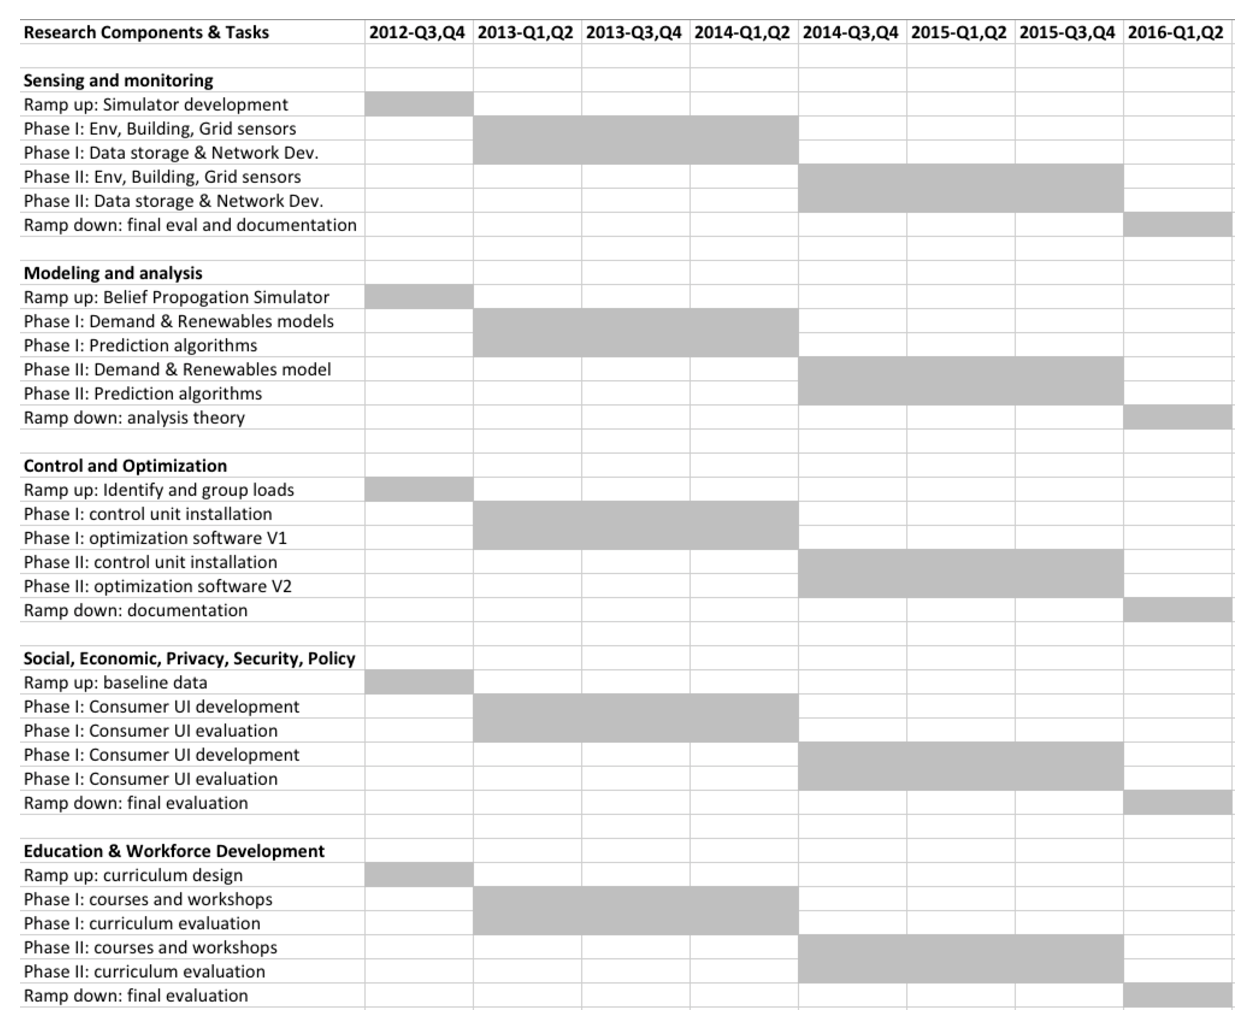
\includegraphics[width=0.9\textwidth]{fig/sep-timeline.eps}
   \caption{Work breakdown structure.}
  \label{fig:timeline}
  \end{center}
\end{figure}

Figure \ref{fig:timeline} illustrates the project timeline, organized by
the five research components.  The four years of this project are broken
down into four phases: a six month ``ramp up'' phase at the start of the
project, followed by two eighteen month phases in which we iteratively
develop and evaluate the microgrid, followed by a six month ``ramp down''
phase in which we focus on documentation, evaluation, and other activities
necessary to allow maximal external use of the knowledge and skills gained
during this project. 

The goal of the initial six month ramp up phase is to complete all of the
startup activities necessary to ensure a successful Phase I implementation
of the microgrid.  For all research components, this involves hiring of
personnel and initial meetings to review literature and become familiar
with relevant issues and technologies. For the sensing and monitoring
component, the ramp up period also involves the development of a simple
server based upon historical data that can provide simulated data about
building loads, environmental data, and grid state.  This simulated data
will be relatively imprecise given the short time available for
implementation, but its goal is to simply enable other research components
to make progress prior to complete installation of sensors.  The modeling
and analysis component will also create a simulator during the ramp up
phase, in this case for a belief propogation network appropriate to the
microgrid. The control and optimization component will research historical
loads and assess control unit types and applicability.   The social,
economic, privacy, security, and policy (SEPSP) research component will
obtain baseline data regarding energy use, attitudes, and concerns
among the university stakeholders. Finally, the education and workforce
development research component will work on curriculum during the ramp up
phase. 

After ramp up, the project begins two eighteen month cycles of microgrid
design, implementation, and evaluation.   We designed the project
so that by the end of year two of this four year project, we will have
created a functional microgrid, though not complete or optimal. 
By the end of Phase I, the sensors and monitoring research component will
have installed an initial set of environmental, grid, and building
sensors and this data will be provided for use in modeling, analysis,
control, and optimization.  Based upon Phase I experiences, the sensors and
monitoring research component will install additional sensors or modify
existing ones to improve the quality of grid performance in Phase II.

A similar iterative approach is employed in the other research
components. During Phase I, the modeling and analysis research component
will create models of both energy demand and renewable resource production
and build an initial prediction algorithm using the data provided by Phase
I sensors and monitoring.  The strengths and weaknesses of these initial
models and the data they are based upon will be evaluated at the end of
Phase I and used to construct more robust and performance models and
prediction algorithms in Phase II.  Similarly, the control and optimization
research component will implement initial control mechanisms during Phase
I, and the results will be used to generate Phase II requirements for the
modeling and analysis and sensors and monitoring research components.   

The SEPSP research component during Phase I and II is similarly iterative,
but here the focus is on creating and evaluating user interfaces that
result in active participation by campus members in the management of the
grid.  Finally, the education and workforce development components will
focus during Phase I on more general curriculum while the micro grid is
still under initial construction.  During Phase II, the curriculum can be
refocused to incorporate ``live'' analysis of the running microgrid and its
operational state. 

The project plan provides for a six month ``ramp down'' period at the
conclusion of the four years.  The goal during this period is to ensure
that we  create curriculum, publications, software, hardware, and
documentation of maximal utility to others wishing to engage in microgrid
development either in Hawaii or on the mainland.   In addition, the final
six months serves as a ``buffer'' period in the event that Phase I or Phase
II takes longer than expected. 








\input{08.project.priornsf}

%%%%%%%%%%%%%%%%%%%%%%%%%%%%%% -*- Mode: Latex -*- %%%%%%%%%%%%%%%%%%%%%%%%%%%%
%% project.conclusions.tex -- 
%% Author          : Philip Johnson
%% Created On      : Fri Jan 13 19:47:12 2012
%% Last Modified By: Philip Johnson
%% Last Modified On: Thu Jan 26 15:45:12 2012
%%%%%%%%%%%%%%%%%%%%%%%%%%%%%%%%%%%%%%%%%%%%%%%%%%%%%%%%%%%%%%%%%%%%%%%%%%%%%%%

\subsection{Conclusions}

In this proposal, we present a vision of a sustainable energy pathway that
begins with the design, implementation, and evaluation of a smart,
sustainable microgrid for the University of Hawaii at Manoa campus.  Our
vision is that the scientific findings, technological innovation, and
social and policy insights gained from this work will contribute to the
ongoing body of work that facilitates the development of microgrids across
the Hawaiian Islands and across the mainland in future years.

The contributions of this research will include the following: (1)
Development of an integrated data collection and management system for both
environmental and energy data; (2) Procedures to determine appropriate
placement of monitoring equipment within a microgrid in order to best
support modeling and control; (3) Analytic techniques for characterizing
the current state of the microgrid without a cost-prohibitive deployment of
sensing equipment; (4) Analytic techniques that enable short-term
prediction of various useful attributes of the microgrid; (5) Automated
techniques for peak shaving/shifting, ramp-rate management, and lowered
overall consumption through control of time-shiftable loads; (6) User
interfaces to enable active participation in energy conservation and
management; (7) Development and evaluation of enhanced security and privacy
mechanisms; (8) Analysis of the cost-benefits of microgrids involving
distributed, intermittent generation; (9) Curriculum and workforce
development for microgrids; and (10) Integration of members of
under-represented minorities.






\newpage

\bibliography{bib/csdl-trs,bib/mf,bib/ref-ak,bib/smartconsumer,bib/sep,bib/tzzt,bib/univcod}
\bibliographystyle{plain}

\end{document}

